\documentclass[12pt]{article}
\usepackage{amssymb, amsmath, amsfonts, bm, graphicx, geometry}
\usepackage{tabularx, booktabs, float, enumitem, multicol, mathtools}
\geometry{margin=1in}


\title{}
\date{}
\author{}

\begin{document}

\begin{titlepage}
    \centering
    \vspace*{1in}

    % Title of the experiment and identifying number
    {\Large\bfseries Lab 2: Verification of the Superposition Principle \par}
    \vspace{1.5cm}

    % Course number
    {\large ESC 221 Basic Principles of Electrical Engineering \par}
    \vspace{2cm}

    % Author's name
    {\large \textbf{Author:} Zeshui Song \par}
    \vspace{0.5cm}

    % Names of other lab group members
    {\large \textbf{Lab Partner:}} \\
    Roy He
    \vfill

    % Date on which the lab was performed
    {\large Date Performed: February 19, 2026 \par}
    \vspace{0.8cm}

    % Name of organization sponsoring the work
    {\large Cooper Union \par}

    \vspace*{1in}
\end{titlepage}
\newpage

\section*{I. Introduction, Experimental Method and Hypotheses}
\textbf{A. Introduction}\\\\
This experiment aims to verify the superposition principle in linear circuits. The superposition principle states that in a linear circuit with multiple independent sources, the voltage or current at any point in the circuit can be found by summing the contributions from each independent source acting individually while all other sources are turned off. \\\\
\textbf{B. Experimental Method}\\\\
In identical resistor networks as shown in Figures \ref{fig:Circuit_A}, \ref{fig:Circuit_B}, and \ref{fig:Circuit_C}, a multimeter will be used to measure the voltages at nodes A and B for voltage sources $V_1$ and $V_2$ individually and then simultaneously. This approach allows for the determination of each source's contribution to the network, which will then be summed to verify the superposition principle for the nodal voltages at A and B in the circuit with both sources active.\\\\
\textbf{C. Hypotheses}\\\\
It is predicted that the measured voltages at nodes A and B in circuit C (Fig. \ref{fig:Circuit_C}) will be equal to the sum of the voltages at nodes A and B in circuits A and B (Figs. \ref{fig:Circuit_A} and \ref{fig:Circuit_B}), thus confirming the superposition principle for this linear circuit network.
\[V_{A_\text{circuit C}} = V_{A_\text{circuit A}} + V_{A_\text{circuit B}}\]
\[V_{B_\text{circuit C}} = V_{B_\text{circuit A}} + V_{B_\text{circuit B}}\]
Based on the nodal analysis calculations shown in the appendix, the predicted nodal voltages for each circuit configuration are as follows:
\begin{itemize}
    \item Circuit A ($V_1$ only): $V_A = 2.2350\,\text{V}$, $V_B = 1.0469\,\text{V}$
    \item Circuit B ($V_2$ only): $V_A = 0.4444\,\text{V}$, $V_B = 2.4002\,\text{V}$
    \item Circuit C ($V_1$ and $V_2$): $V_A = 2.6803\,\text{V}$, $V_B = 3.4476\,\text{V}$
\end{itemize}

\newpage
\section*{II. Equipment List}
\begin{enumerate}
    \item \textbf{Digital Multimeter} \\ 
          Manufacturer: AstroAI \\
          Model: AM33B
    \item \textbf{DC Power Supply} \\ 
          Manufacturer: GW Instek \\
          Model: SPD-3606
\end{enumerate}
\newpage
\section*{III. Wiring / Schematic Diagram / Procedure}
\textbf{A. Procedure}\\\\
1. Constructing Circuit A
\begin{enumerate}
    \item A circuit was constructed as illustrated in Fig.~\ref{fig:Circuit_A} using a DC power supply ($V_1 = 5\,\text{V}$) and resistors ($R_1 = 1k\,\Omega$, $R_2 = 1k\,\Omega$, $R_3 = 2.2k\,\Omega$, $R_4 = 3.3k\,\Omega$, and $R_5 = 4.7k\,\Omega$).
    \item Resistor $R_1$ was connected between the positive terminal of $V_1$ and node A.
    \item Resistor $R_2$ was connected between node A and ground.
    \item Resistor $R_3$ was connected between node A and node B.
    \item Resistor $R_4$ was connected between node B and ground.
    \item Resistor $R_5$ was connected between node B and ground.
    \item The negative terminal of $V_1$ was connected to ground.
\end{enumerate}
2. Constructing Circuit B
\begin{enumerate}
    \item A circuit was constructed as illustrated in Fig.~\ref{fig:Circuit_B} using a DC power supply ($V_2 = 10\,\text{V}$) and resistors ($R_1 = 1k\,\Omega$, $R_2 = 1k\,\Omega$, $R_3 = 2.2k\,\Omega$, $R_4 = 3.3k\,\Omega$, and $R_5 = 4.7k\,\Omega$).
    \item Resistor $R_1$ was connected between node A and ground.
    \item Resistor $R_2$ was connected between node A and ground.
    \item Resistor $R_3$ was connected between node A and node B.
    \item Resistor $R_4$ was connected between node B and ground.
    \item Resistor $R_5$ was connected between node B and the negative terminal of $V_2$.
    \item The negative terminal of $V_2$ was connected to ground.
\end{enumerate}
3. Constructing Circuit C
\begin{enumerate}
    \item A circuit was constructed as illustrated in Fig.~\ref{fig:Circuit_C} using both DC power supplies ($V_1 = 5\,\text{V}$ and $V_2 = 10\,\text{V}$) and resistors ($R_1 = 1k\,\Omega$, $R_2 = 1k\,\Omega$, $R_3 = 2.2k\,\Omega$, $R_4 = 3.3k\,\Omega$, and $R_5 = 4.7k\,\Omega$).
    \item Resistor $R_1$ was connected between the positive terminal of $V_1$ and node A.
    \item Resistor $R_2$ was connected between node A and ground.
    \item Resistor $R_3$ was connected between node A and node B.
    \item Resistor $R_4$ was connected between node B and ground.
    \item Resistor $R_5$ was connected between node B and the negative terminal of $V_2$.
    \item The negative terminals of $V_1$ and $V_2$ were both connected to ground.
\end{enumerate}
4. Measurements and Data Collection
\begin{enumerate}
    \item For each circuit configuration (A, B, and C), the voltages at nodes A and B were measured using a multimeter with the positive lead connected to nodes A and B, respectively, and the negative lead connected to ground.
\end{enumerate}
\newpage\noindent
\textbf{B. Schematic Diagram}
\begin{figure}[H]
    \centering
    
\includegraphics[width=0.8\linewidth]{Circuit A.png}
    \caption{Circuit A: A DC circuit network consisting of a fixed voltage source $V_1$ and resistors $R_1$, $R_2$, $R_3$, $R_4$, and $R_5$ with labeled nodes A and B for measurement points.}
    \label{fig:Circuit_A}
\end{figure}
\begin{figure}[H]
    \centering
    
\includegraphics[width=0.8\linewidth]{Circuit B.png}
    \caption{Circuit B: A DC circuit network consisting of a fixed voltage source $V_2$ and resistors $R_1$, $R_2$, $R_3$, $R_4$, and $R_5$ with labeled nodes A and B for measurement points.}
    \label{fig:Circuit_B}
\end{figure}
\begin{figure}[H]
    \centering
    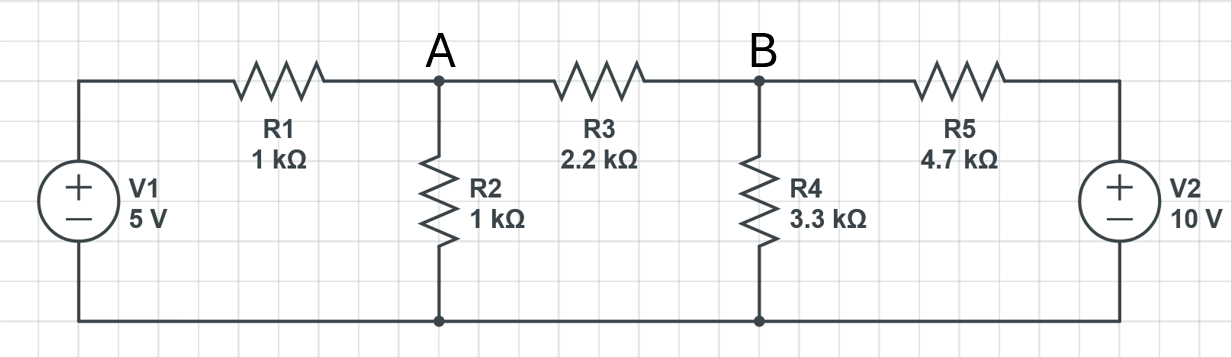
\includegraphics[width=0.8\linewidth]{Circuit C.png}
    \caption{Circuit C: A DC circuit network consisting of both voltage sources $V_1$ and $V_2$ and resistors $R_1$, $R_2$, $R_3$, $R_4$, and $R_5$ with labeled nodes A and B for measurement points.}
    \label{fig:Circuit_C}
\end{figure}
\newpage
\section*{IV. Results}
\begin{table}[H]
\centering
\caption{Comparison of Calculated and Measured Nodal Voltages}
\begin{tabularx}{\linewidth}{*{4}{>{\centering\arraybackslash}X}}
\toprule
\textbf{Nodal Voltage (V)} & \textbf{Circuit A ($V_1$=5V)} & \textbf{Circuit B ($V_2$=10V)} & \textbf{Circuit C ($V_1$ \& $V_2$)} \\
\midrule
\textit{Calculated Values} & & & \\
V$_A$  & 2.2350 & 0.4444 & 2.6803 \\
V$_B$  & 1.0469 & 2.4002 & 3.4476 \\
\midrule
\textit{Measured Values} & & & \\
V$_A$  & 2.29 & 0.43 & 2.75 \\
V$_B$  & 1.04 & 2.34 & 3.38 \\
\bottomrule
\end{tabularx}
\end{table}
\newpage
\section*{V. Discussion, Analysis and Concluding Statements}
\textbf{A. Verification of Superposition with Calculated Values}\\\\
Comparing the calculated nodal voltages for circuits A, B, and C using nodal analysis, the sum of the voltages at nodes A and B for circuits A and B closely matches the calculated voltages for circuit C (some difference due to rounding), confirming the superposition principle.
\[V_{A_\text{circuit C}} = V_{A_\text{circuit A}} + V_{A_\text{circuit B}}\]
\[\implies 2.6803\,\text{V} \approx 2.2350\,\text{V} + 0.4444\,\text{V}= 2.6794\,\text{V}\]
\[V_{B_\text{circuit C}} = V_{B_\text{circuit A}} + V_{B_\text{circuit B}}\]
\[\implies 3.4476\,\text{V} \approx 1.0469\,\text{V} + 2.4002\,\text{V}= 3.4471\,\text{V}\]
\textbf{B. Verification of Superposition with Measured Values}\\\\
Comparing the measured nodal voltages for circuits A, B, and C in Table 1, the sum of the voltages at nodes A and B for circuits A and B closely matches the measured voltages for circuit C, confirming the superposition principle in practice.
\[V_{A_\text{circuit C}} = V_{A_\text{circuit A}} + V_{A_\text{circuit B}}\]
\[\implies 2.75\,\text{V} \approx 2.29\,\text{V} + 0.43\,\text{V}= 2.72\,\text{V}\]
\[V_{B_\text{circuit C}} = V_{B_\text{circuit A}} + V_{B_\text{circuit B}}\]
\[\implies 3.38\,\text{V} \approx 1.04\,\text{V} + 2.34\,\text{V}= 3.38\,\text{V}\]
\textbf{C. Conclusion}\\\\
This experiment successfully verified the superposition principle in linear circuits. Both the calculated and measured nodal voltages at nodes A and B for circuit C closely matched the sum of the voltages from circuits A and B, confirming that the contributions from each independent source can be linearly added to determine the overall response in a linear circuit network. Small discrepancies in the verification of superposition with measured values can be attributed to factors such as resistor tolerances, fluctuations in the voltage readings, and measurement uncertainties. Overall, the results support the validity of the superposition principle.
\newpage
\section*{VI. Appendix}
\textbf{Calculations for Predicated Nodal Voltages}\\\\
Using nodal analysis, the predicted voltages at nodes A and B for circuits A, B, and C can be calculated as follows : \\\\
\textbf{A. Circuit A}\\
Using $V_1 = 5\,\text{V}$, $R_1 = 1k\,\Omega$, $R_2 = 1k\,\Omega$, $R_3 = 2.2k\,\Omega$, $R_4 = 3.3k\,\Omega$, and $R_5 = 4.7k\,\Omega$.\\
1. Node A KCL Equation:
\[\frac{V_1-V_A}{R_1} = \frac{V_A-V_B}{R_3} + \frac{V_A}{R_2} \implies 0.005 = 0.00245V_A -0.0004545V_B\]
2. Node B KCL Equation:
\[\frac{V_A-V_B}{R_3} = \frac{V_B}{R_4} + \frac{V_B}{R_5}\implies 0 = 0.0004545V_A -0.0009703V_B\]
Solving the system of equations yields:
\[V_A = 2.2350\,\text{V}\]
\[V_B = 1.0469\,\text{V}\]
\textbf{B. Circuit B}\\
Using $V_2 = 10\,\text{V}$, $R_1 = 1k\,\Omega$, $R_2 = 1k\,\Omega$, $R_3 = 2.2k\,\Omega$, $R_4 = 3.3k\,\Omega$, and $R_5 = 4.7k\,\Omega$.\\
1. Node B KCL Equation:
\[\frac{V_2 - V_B}{R_5} = \frac{V_B}{R_4} + \frac{V_B-V_A}{R_3}\implies 0.002127= -0.0004545V_A + 0.0009703V_B\]
2. Node A KCL Equation:
\[\frac{V_B-V_A}{R_3} = \frac{V_A}{R_2} + \frac{V_A}{R_1}\implies 0 = 0.0024545V_A -0.0004545V_B\]
Solving the system of equations yields:
\[V_A = 0.4444\,\text{V}\]
\[V_B = 2.4002\,\text{V}\]
\textbf{C. Circuit C}\\
Using $V_1 = 5\,\text{V}$, $V_2 = 10\,\text{V}$, $R_1 = 1k\,\Omega$, $R_2 = 1k\,\Omega$, $R_3 = 2.2k\,\Omega$, $R_4 = 3.3k\,\Omega$, and $R_5 = 4.7k\,\Omega$.\\
1. Node A KCL Equation:
\[\frac{V_1 - V_A}{R_1} = \frac{V_A - V_B}{R_3} + \frac{V_A}{R_2}\implies 0.005 = 0.00245V_A -0.0004545V_B\]
2. Node B KCL Equation:
\[\frac{V_A - V_B}{R_3} = \frac{V_B}{R_4} + \frac{V_B-V_2}{R_5}\implies -0.002127= 0.0004545V_A - 0.0009703V_B\]
Solving the system of equations yields:
\[V_A = 2.6803\,\text{V}\]
\[V_B = 3.4476\,\text{V}\]

\end{document}